\chapter{Introdução}

Com o passar dos anos, o mercado demanda e espera software inovadores e de alta qualidade, que sejam adequados a suas necessidades $-$ e o mais rápido possível \cite{TheBusinessOfInnovation}.

O desenvolvimento ágil de software, que neste ano de 2012 completa 11 anos, foi elaborado \cite{AgileManifesto} visando atender à estas expectativas do mercado, focando o processo de desenvolvimento nas pessoas e abraçando as mudanças que  naturalmente surgem durante a construção do software. De acordo com \citeonline{PMNetworkFailureDrop}, o \textit{Chaos Manifesto 2011}\footnote{O \textit{Chaos Manifesto} é uma pesquisa bienal realizada pelo \textit{The Standish Group} e teve início em 1994. As pesquisas publicadas em um ano representam os dados do ano anterior.} mostra que os resultados de 2010 representam, desde sua primeira edição, a maior taxa de sucesso nos projetos de desenvolvimento de software, que aumentou de 32\% em 2008 para 37\% em 2010. Segundo \citeonline{ResumoChaosReport}, o \textit{The Standish Group} conclui que uma das razões para o aumento da taxa de sucesso foi a utilização das metodologias ágeis, que cresce a uma taxa de 22\% CAGR\footnote{\href{http://en.wikipedia.org/wiki/Compound_annual_growth_rate} {Compound annual growth rate}} e hoje são adotados em 9\% de todos os projetos de Tecnologia da Informação em andamento e em 29\% dos novos projetos.

Como a adoção do desenvolvimento ágil é crescente nos últimos anos, diversos métodos e técnicas vem sendo desenvolvidos tendo como base os princípios e valores ágeis \cite{BDDRodrigo}, principalmente relacionadas ao teste de software e que serão abordadas no presente trabalho, sendo elas o Desenvolvimento Guiado por Testes (do inglês, \textit{Test-Driven Development} - TDD), Desenvolvimento Guiado por Comportamento (do inglês, \textit{Behaviour-Driven Development - BDD}), Integração Contínua e Dublês de Teste. Sendo técnicas emergentes, ainda são pouco discutidas no meio acadêmico, este trabalho pretende contribuir com esta discussão e, de certa forma, introduzir estas técnicas emergentes na academia.


\section{Justificativas e objetivos}

Existem poucos trabalhos acadêmicos no que se refere a técnicas emergentes de testes de software, como notado também por \citeonline{BDDSolis}, que em 2011 foram os primeiros a ter um artigo publicado sobre Desenvolvimento Guiado por Comportamento (BDD), pela \textit{IEEE Computer Society}.

Sendo assim, o objetivo do presente trabalho é contribuir com a introdução de técnicas e discussões surgidas no meio empresarial para a academia, além de agregar conhecimentos, ora dispersos e difusos, sobre as diferentes abordagens, possibilidades e pontos em aberto no emprego de tais técnicas.

As técnicas que serão abordadas neste trabalho tem seu conceito definido no mercado e evoluem através da evolução das ferramentas que os implementam. O fluxo de evolução é o seguinte:

\begin{itemize}
  \item Cria-se um conceito e uma ferramenta que o implemente.
  \item Com base na utilização e observação desta ferramenta, há uma percepção de novas necessidades, fazendo que novas ferramentas sejam criadas e que os conceitos evoluam.
\end{itemize}

Desta forma, a evolução das ferramentas e a evolução conceitual estão intimamente ligadas. No texto original sobre BDD \cite{IntroducingBDD} já se encontra isto. A inspiração para a criação de BDD foi uma ferramenta chamada \textit{AgileDox}\footnote{Mais informações em \url{http://agiledox.sourceforge.net}}, que fez o autor antever as novas possibilidades que cristalizou no conceito de BDD. Justamente por esta característica dinâmica, a informação e os diferentes conceitos estão dispersos, pois nunca foram sistematizados, ficando em uma espécie de ``inteligência coletiva"\ da comunidade de desenvolvimento ágil.

Além disso, como o presente trabalho está no contexto dos métodos ágeis, e nestes as partes conceitual e prática formam um todo inseparável, para toda técnica abordada serão utilizados exemplos mostrando código de um projeto real.

\section{Metodologia}

Será feita uma explanação sobre cada técnica e uma discussão comparando as diferentes abordagens, possibilidades e pontos em aberto no emprego de cada técnica.

Como base para a discussão, será utilizado o kanban-roots\footnote{\url{http://github.com/hugomaiavieira/kanban-roots}}, que está foi desenvolvido pelo autor.

O kanban-roots é um kanban\footnote{O termo tem origem no sistema Toyota de produção, onde kanban é a maneira como é coordenado o fluxo de peças na cadeia de suprimentos  \cite{AMaquinaQueMudouOMundo}. No contexto do presente trabalho, kanban é um quadro para visualização do fluxo de trabalho (tarefas) em um projeto.} online para auxiliar a organização e acompanhamento das tarefas em um projeto, sendo especialmente interessante para projetos \textit{opensouce} ou, de modo geral, para projetos com equipes geograficamente distribuídas. O kanban-roots já está em produção e vem sendo testado e utilizado com sucesso por algumas pessoas em empresas do Brasil como a Algorich, Voxline, Mandic, Quatix, mas também estrangeiras como a infoPiiaf e Free.fr (França), Ginzametrics (Estados Unidos), Osube (China), Centah (Canadá), Podmoskovie.info (Rússia), EvoEnergy (Inglaterra), Forgotten Labs (Lituânia), entre outros.

Na figura \ref{img:tela_kaban_roots} pode ser visto um \textit{print} da tela do kanban de um projeto no kanban-roots.

\begin{figure}[h]
  \center
  \caption{Tela do kanban de um projeto no kanban-roots}
  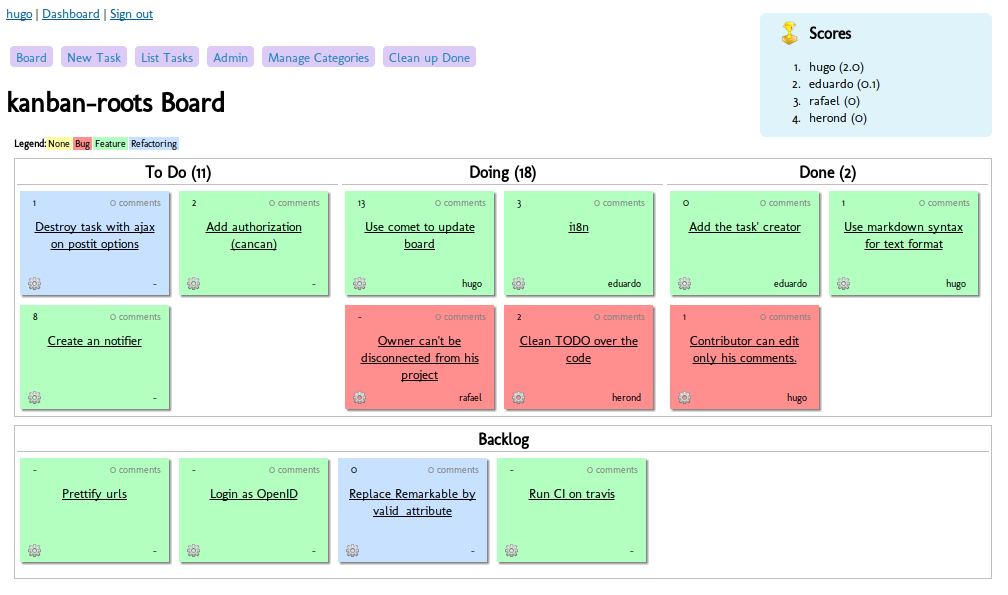
\includegraphics[scale=0.45]{images/kanban-roots}
  \label{img:tela_kaban_roots}
\end{figure}

Todos os trechos de código apresentados neste trabalho são trechos retirados do kanban-roots. A primeira linha de cada trecho sempre é um comentário informando o nome do arquivo original.

\section{Ferramentas utilizadas}

Para o desenvolvimento do kanban-roots foram utilizadas diversas ferramentas, sendo importante citar em que contexto e momento cada uma delas é utilizada.

Como base para o desenvolvimento, foi utilizado o \textit{framework web} Ruby On Rails\footnote{\url{http://rubyonrails.org}}. Para os testes de unidade apresentados na Seção \ref{sec:tdd} foi utilizado o Test::Unit\footnote{\url{http://test-unit.rubyforge.org/}}. Já na Seção \ref{sec:bdd} é utilizado o Rspec\footnote{\url{http://rspec.info/}} para testes unitários, testes de aceitação e dublês de teste. Ainda na Seção \ref{sec:bdd} também foi utilizado o Cucumber\footnote{\url{http://cukes.info/}} para testes de aceitação. Além dessas ferramentas, também foi utilizado o FactoryGirl\footnote{\url{https://github.com/thoughtbot/factory_girl}} para \textit{fixtures replacement} em todos os momentos em que se fez necessário.

\section{Trabalhos relacionados} % (fold)
\label{sec:trabalhos_relacionados}

Não existem muitos trabalhos acadêmicos relacionados às técnicas abordadas no presente trabalho, e todos eles abordam o tema apenas conceitualmente, deixando uma lacuna em termos de contextualização.

\citeonline{BDDSolis} apresentam algumas das principais características do \textit{Behaviour-Driven Development} (BDD), tendo como base uma pequena quantidade de estudo publicados sobre o tema e as ferramentas existentes para a utilização da técnica.

Sobre \textit{Test-Driven Development} (TDD), praticamente são apenas encontrados estudos empíricos, com estudos de caso na academia e na indústria, que discutem a efetividade do uso do TDD. Na Seção \ref{sub:a_efetividade_do_tdd} será feita uma análise destes estudos.

% section trabalhos_relacionados (end)

